\section{The Linear Growth of the Residual States}
\label{appsec:res-peak}

\subsection{The minimal model structure to recapitulate residual state peak}
\label{appsec:mini-res-peak}
We give more details for the claim in Section~\ref{sec:res-peak}, stating that ``The residual-state peaks require a three-layer structure.''
Figure~\ref{appfigure:massive_minimal} presents the difference of residual norms between the \bos~token and others ($\|\res_{\bos}\|-\E_{\tok\neq\bos}[\|\res_{\tok}\|]$), with different combinations of model structures. The $3\times \TF$ and $2\times \TF+\mlp$ are the architectures that demonstrate clear evidence of residual state peaks. 

\begin{figure}[h]
    \centering
    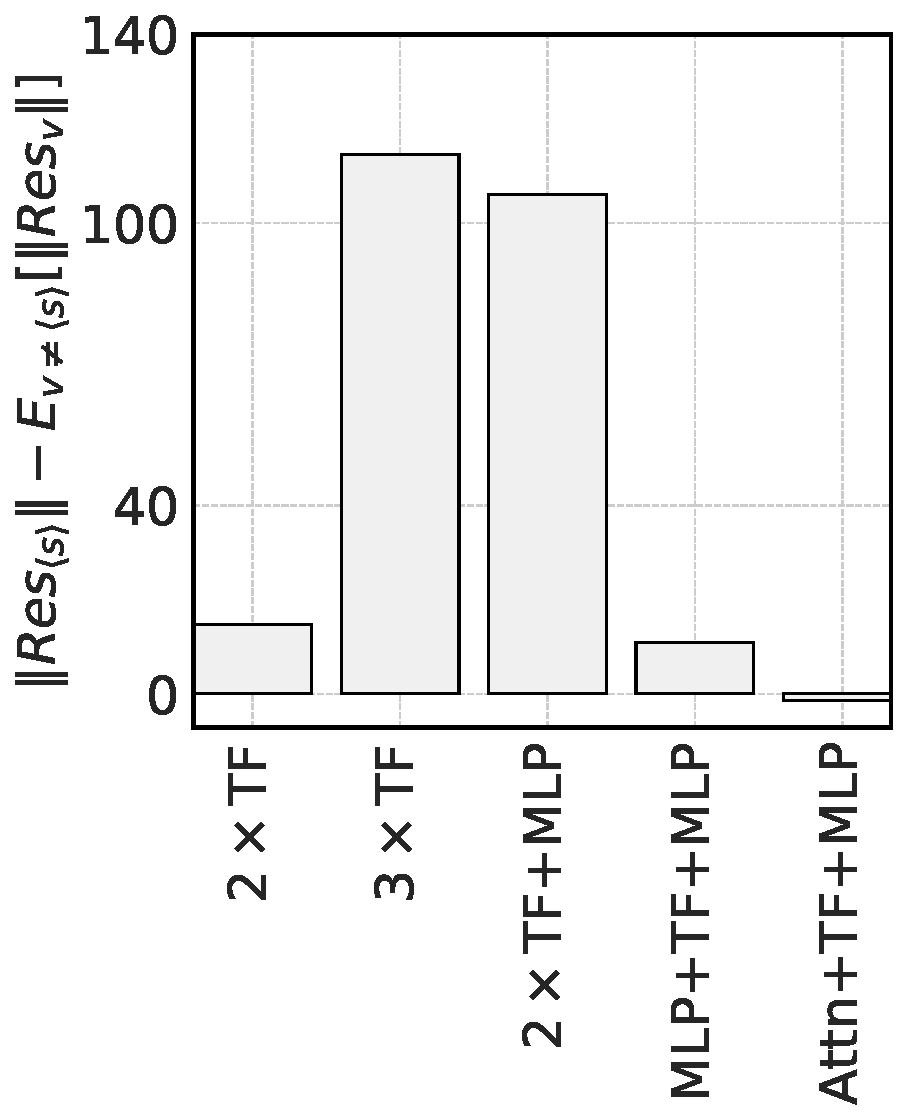
\includegraphics[width=0.3\linewidth]{Figures/BBM_appendix/massive_norm_minimal.pdf}
    \caption{\small Minimal structures to elicit residual state peaks. We use $A+B+C$ to indicate the model with structure $A$, $B$, $C$ in layers 0, 1, and 2, respectively.}
    \label{appfigure:massive_minimal}
\end{figure}



\subsection{Additional plots for the three-layer transformer trained on BB task}
\label{appsec:three-layer-tf}
We provide more results to the three layer transformer model trained on the BB task. They provide supporting evidence for the claim in Section~\ref{sec:res-peak}, stating that “Massive residual states amplify attention sinks and value-state drains in later layers.”
Figures \ref{appfigure:massive-attn}, \ref{appfigure:massive-value-norm}, and \ref{appfigure:massive-norm} show the extreme token phenomena in a three-layer transformer. The residual state peaks show different phenomena from those in LLMs, with the last layer output increasing the residual norms of non-\bos~tokens. Figure \ref{figure:extreme-token}
 demonstrates that the residual state norms of \bos~drop match the magnitudes of other tokens at the last layer. 
\begin{figure}[h]
  \centering
  \begin{minipage}{0.3\textwidth}
      \centering
      \subcaption{\small Layer 0}
      \vspace{-.2em}
      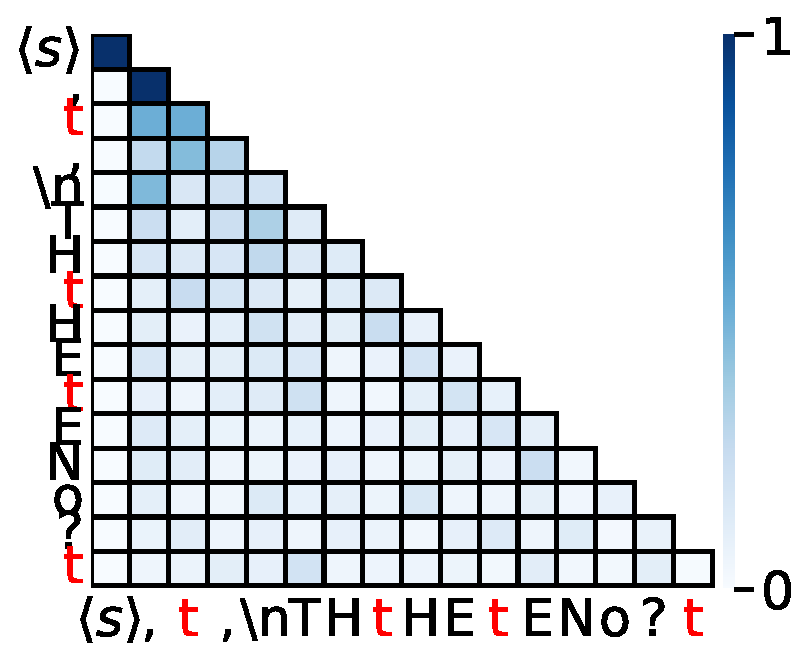
\includegraphics[width=\linewidth]{Figures/BBM_appendix/massive_attn_step10k_fig0.pdf}
  \end{minipage}
  % \hspace{-1em}
  \begin{minipage}{0.3\textwidth}
      \centering
      \subcaption{\small Layer 1}
      \vspace{-.2em}
      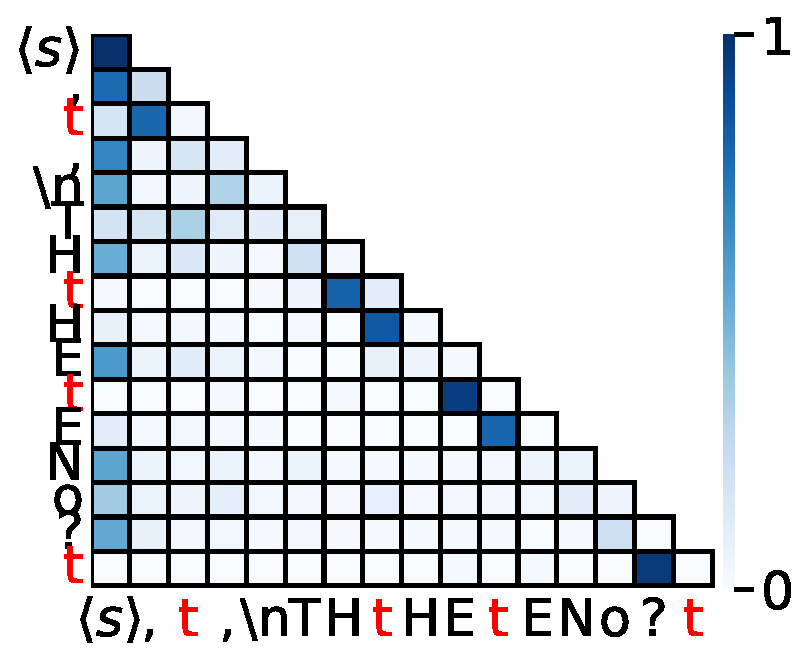
\includegraphics[width=\linewidth]{Figures/BBM_appendix/massive_attn_step10k_fig1.pdf}
  \end{minipage}
  % \hspace{-1em}
  \begin{minipage}{0.3\textwidth}
      \centering
      \subcaption{\small Layer 2}
      \vspace{-.2em}
      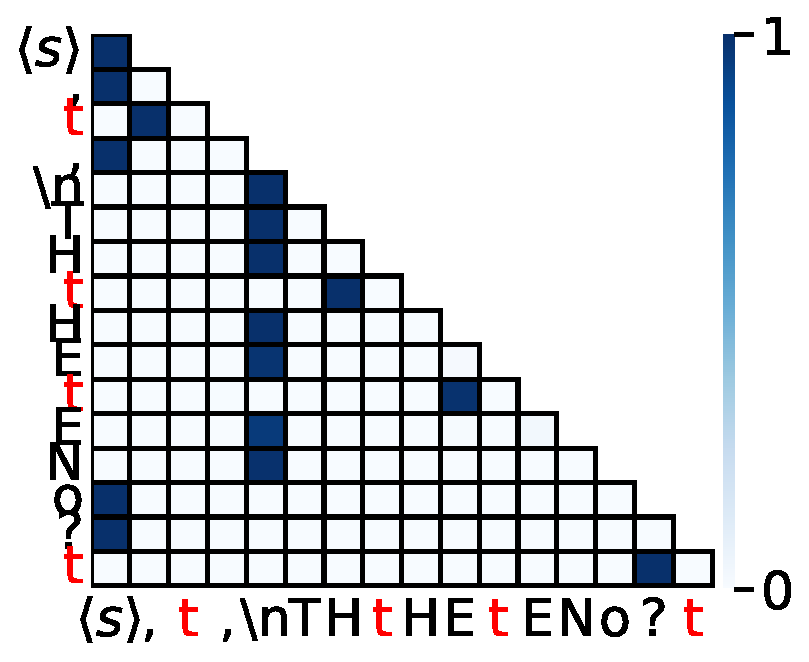
\includegraphics[width=\linewidth]{Figures/BBM_appendix/massive_attn_step10k_fig2.pdf}
  \end{minipage}
  % \vspace{-1em}
  \caption{\small Attention weight patterns of three-layer transformer trained on the BB task}
  \label{appfigure:massive-attn}
  \vspace{-1em}
\end{figure}

\begin{figure}[h]
  \centering
  \begin{minipage}{0.3\textwidth}
      \centering
      \subcaption{\small Layer 0}
      \vspace{-.2em}
      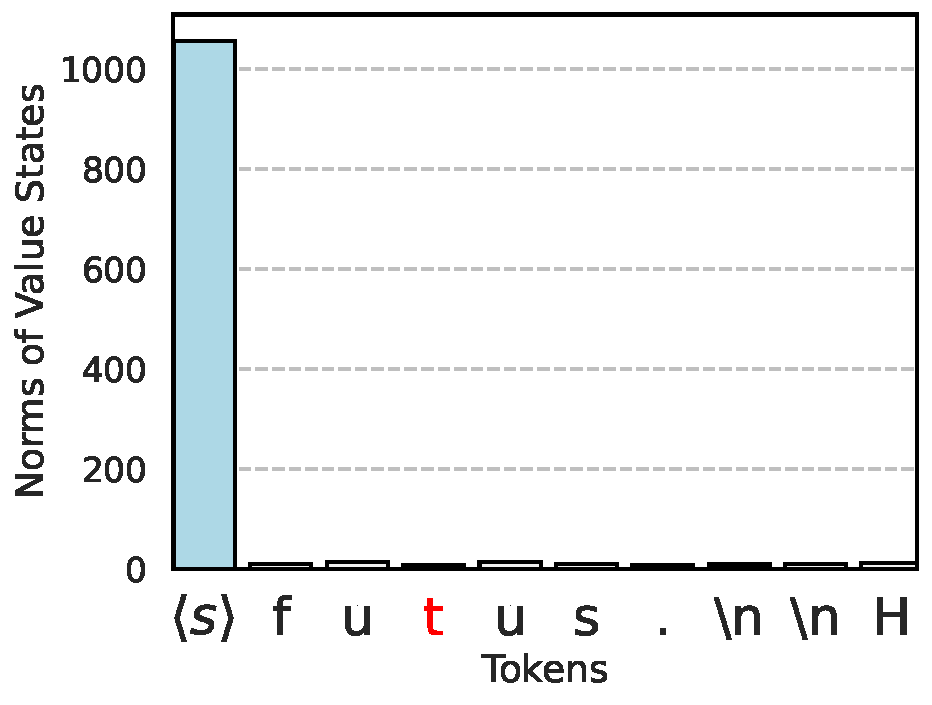
\includegraphics[width=\linewidth]{Figures/BBM_appendix/value_states_layer_0.pdf}
  \end{minipage}
  % \hspace{-1em}
  \begin{minipage}{0.3\textwidth}
      \centering
      \subcaption{\small Layer 1}
      \vspace{-.2em}
      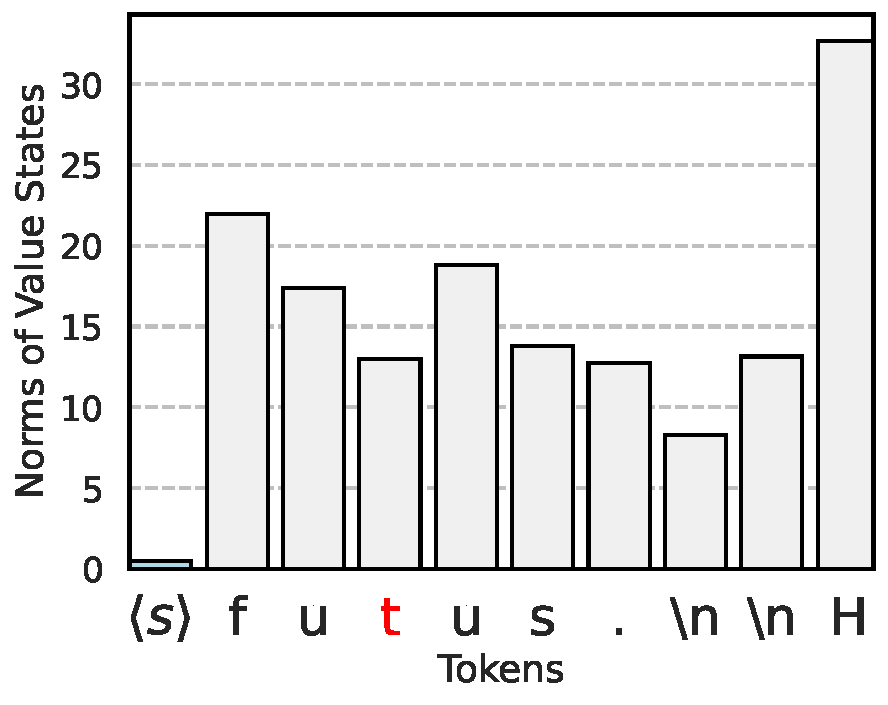
\includegraphics[width=\linewidth]{Figures/BBM_appendix/value_states_layer_1.pdf}
  \end{minipage}
  % \hspace{-1em}
  \begin{minipage}{0.3\textwidth}
      \centering
      \subcaption{\small Layer 2}
      \vspace{-.2em}
      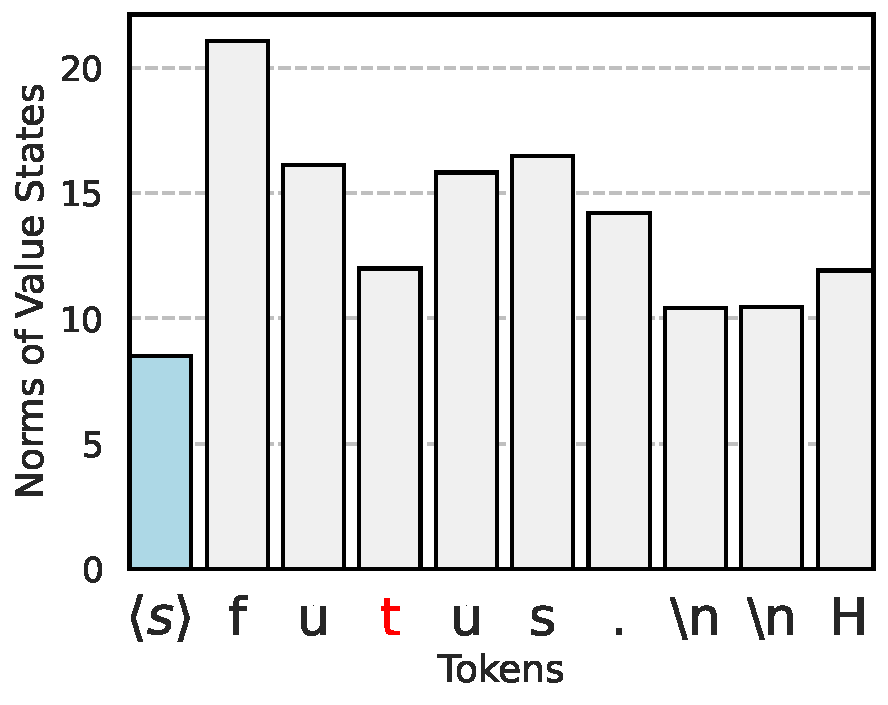
\includegraphics[width=\linewidth]{Figures/BBM_appendix/value_states_layer_2.pdf}
  \end{minipage}
  % \vspace{-1em}
  \caption{\small Value state norms of three-layer transformer trained on the BB task}
  \label{appfigure:massive-value-norm}
  \vspace{-1em}
\end{figure}


\begin{figure}[h]
  \centering
  \begin{minipage}{0.3\textwidth}
      \centering
      \subcaption{\small Layer 0}
      \vspace{-.2em}
      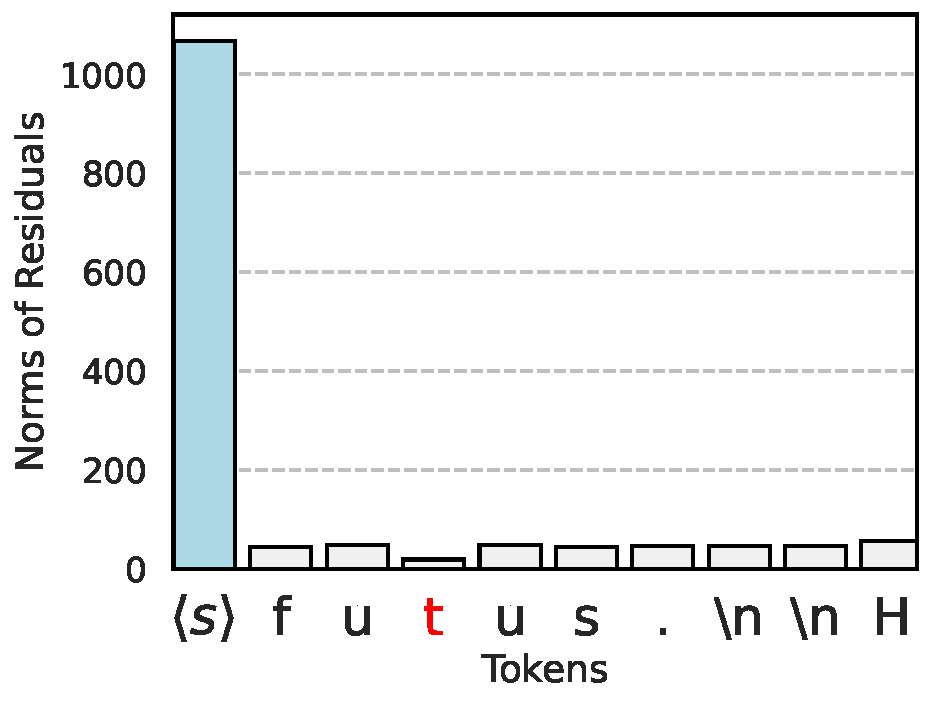
\includegraphics[width=\linewidth]{Figures/BBM_appendix/norms_layer_0.pdf}
  \end{minipage}
  % \hspace{-1em}
  \begin{minipage}{0.3\textwidth}
      \centering
      \subcaption{\small Layer 1}
      \vspace{-.2em}
      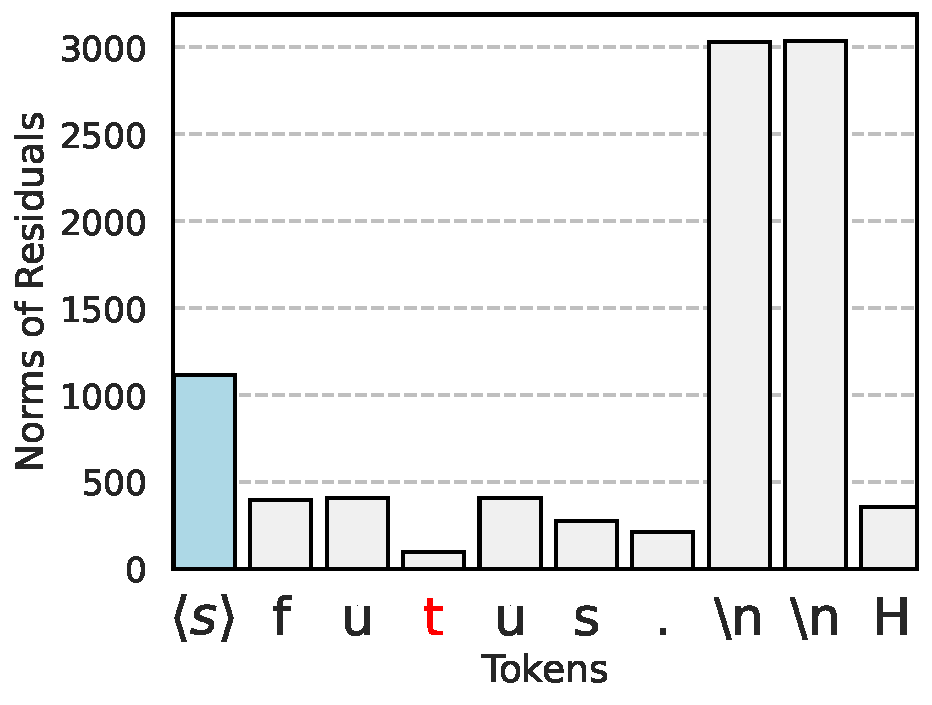
\includegraphics[width=\linewidth]{Figures/BBM_appendix/norms_layer_1.pdf}
  \end{minipage}
  % \hspace{-1em}
  \begin{minipage}{0.3\textwidth}
      \centering
      \subcaption{\small Layer 2}
      \vspace{-.2em}
      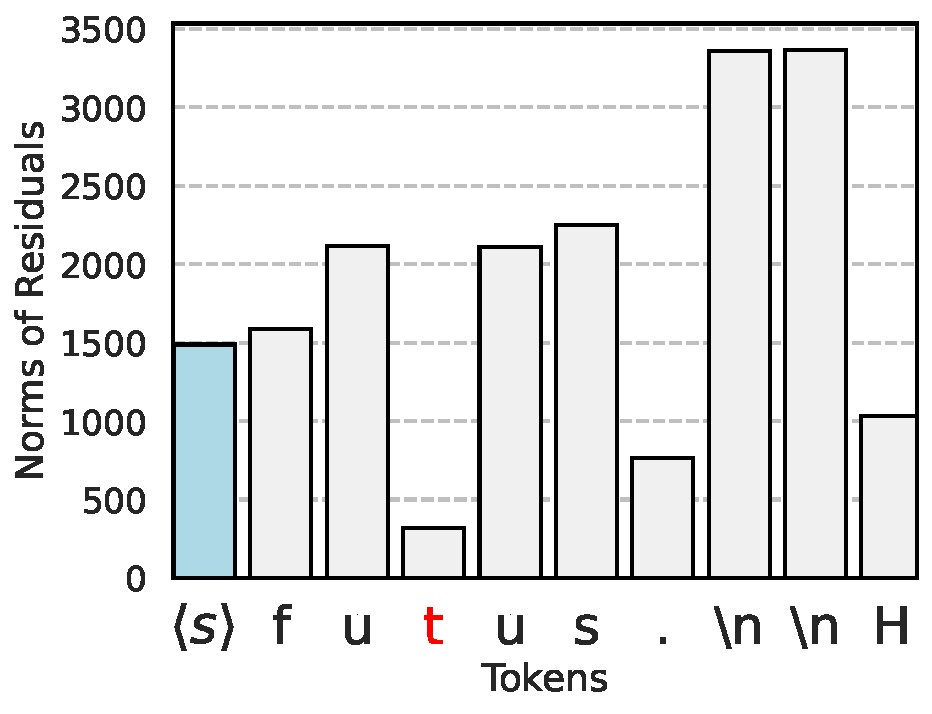
\includegraphics[width=\linewidth]{Figures/BBM_appendix/norms_layer_2.pdf}
  \end{minipage}
  % \vspace{-1em}
  \caption{\small Residual state norms of three-layer transformer trained on the BB task}
  \label{appfigure:massive-norm}
  \vspace{-1em}
\end{figure}


\subsection{Potential mechanism for linear growth of the residual state peak in multi-layer models}
\label{appsec:theory-for-res}
We give more details for the claim in Section~\ref{sec:res-peak}, stating that ``The ReLU attention and changing Adam to SGD eliminates the residual state peaks'' We first state Claim~\ref{sec:res-peak}.
\begin{claim}[Potential mechanism for the formation of residual-state peaks]\label{claim:res-peak}
In the training dynamic of a multi-layer transformer, if the mutual reinforcement mechanism (cf.\ Claim~\ref{claim:mutual-reinforcement}) occurs in upper layers:
\begin{enumerate}
    \item The gradients of $\res_\bos$ have the same direction (aligning with the null space of value matrices in upper layers and the $\key_\bos$) along the training dynamics.
    \item The layer-norm operations cause the fast decay of the magnitude of the gradients.
    \item Adam induces diminishing gradients to be constant updates, leading to the linear growth for the norm of the residual state of the extreme token.
\end{enumerate}
\end{claim}
To support the claim, we use the simplified model in Section~\ref{sec:bb_task}, including the residual state norm.
Denote the layer-norm operation as $\lnm$.
Heuristically, we can split the residual state $\res_{\bos}$ to a summation of two directions.
\[
\res_{\bos} = m \cdot \bm{\eta} + \bm{\eps},
\]
where $\bm{\eta},\bm{\eps} \in \R^\vocabsize$ with $\|\bm{\eta}\|_2=\|\bm{\eps}\|_2 = 1$, and $\bm{\eta}^\top \bm{\eps} = \rho>0$. The $\bm{\eta}$ corresponds to the direction of $\key_\bos$ in the original transformer, and $\bm{\eps}$ corresponds to other directions.
Assume that the attention logit from the token $\tok$ to the \bos~token in layer 1 is given by 
\begin{equation}\label{eqn:logits_in_residual_massive} \text{logit}_{\tok,\bos}= \sink_\tok = \Tilde{\sink}_\tok \bm{\eta}^\top \lnm(\res_{\bos})=\Tilde{\sink}_\tok \cdot \frac{m+\rho}{\sqrt{m^2+2m\rho+1}}.\end{equation}
We assume that the scalars $m$ and $\Tilde{\sink}$ are trainable, quantifying the norm of the residual states and magnitude of attention sinks. In the loss function $\loss_\tok$ as defined in Eq.~\eqref{eqn:loss_single}, we replace $\sink_\tok$ by the expression as in Eq.~(\ref{eqn:logits_in_residual_massive}), so that the loss function becomes a function of $(\Tilde{\sink}_\tok, \vecvalue, m)$, denoted as
\[
\wt{\loss}_\tok(\Tilde{\sink}_\tok, \vecvalue, m) = \loss_\tok(\sink_\tok, \vecvalue),
\]
We then consider the total loss as the average of the losses on each non-trigger token, weighted by its proportion in the stable distribution $\{\pi_v\}_{v \in \vocab}$, given by
\begin{equation}\label{appeqn:res_total_loss}
\wt{\loss}(\Tilde{\vecsink}, \vecvalue, m) = \sum_{\tok \in \vocab \setminus \cT} \stable_\tok \cdot \wt{\loss}_\tok(\Tilde{\sink}_\tok, \vecvalue, m).
\end{equation}
\begin{proposition}\label{appthm:massive}
% Consider the gradient flow of the loss function $\wt{\loss}(\Tilde{\vecsink}, \vecvalue, m)$. 
Assume $\xi_\tok\geq 0$ for any $\tok$, $\set{W_k\ivalue_k}_{k\in\vocab}$ are not all equal, and $\rho>0$. Fix $\vecvalue=\bm{0}$, and consider the gradient flow of $\wt{\loss}(\Tilde{\vecsink}, \vecvalue, m)$ over $\Tilde{\vecsink}$ and $m$. With any initial value $\Tilde{\sink}_\tok(0)>0$ for any $\tok$ and $m(0)>0$, we have that
\[
\dot{m}(t)=O\Big(\frac{\log t}{\sqrt{t} m^{3}}\Big).
\]
\end{proposition}
\begin{proof}[Proof of Proposition~\ref{appthm:massive}]
The chain rule gives that
\[
\dot{\Tilde{\sink}}_\tok(t) = \dot{\sink}_\tok \cdot \frac{m+\rho}{\sqrt{m^2+2m\rho+1}},
\]
and
\[
\dot{m}(t) = \sum_{\tok=1}^\vocabsize \Big\{\dot{\sink}_\tok \Tilde{\sink}_\tok \cdot \frac{\mathrm{d} \lnm(\res_\bos)}{\mathrm{d} t} \Big\}.
\]
With the initial values, $\dot{m}(t)\geq 0$ and $\dot{\Tilde{\sink}}_\tok(t) \geq 0$.
We have $m(t)\geq 0$ for any $t$. Hence, $$\dot{\Tilde{\sink}}_\tok \in [\rho \dot{\sink}_\tok,  \dot{\sink}_\tok].$$ 
Therefore, $\Tilde{\vecsink} = 2^\inv \log t \bm{1} + \Tilde{\bm{r}}(t)$ with $\Tilde{\bm{r}}(t)$ uniformly bounded over time. Furthermore, we have that
\begin{align*}
\dot{m}(t) & = \sum_{\tok=1}^\vocabsize \Big\{\dot{\sink}_\tok \Tilde{\sink}_\tok \cdot \frac{\mathrm{d} \lnm(\res_\bos)}{\mathrm{d} t} \Big\}\\
& = O\Big(\frac{\log t}{\sqrt{t}}\Big) \cdot \frac{1-\rho^2}{(m^2+2m\rho+1)^{3/2}}\\
& = O\Big(\frac{\log t}{\sqrt{t}m^3}\Big).
\end{align*}
This proves Proposition~\ref{appthm:massive}.
\end{proof}
We use simulation to demonstrate the effect of Adam. We train the scalar $m$ using Adam with gradient $\mathrm{d}m = \log t / [\sqrt{t}m^3]$. We set $\beta_1=0.9$, $\beta_2=0.999$, weight decay$=10^{-8}$, and the learning rate $\text{lr}=0.3$. Figure~\ref{appfigure:m_dynamics} presents the training dynamics of $m$. We observe the linear growth after a warming-up phase. In contrast, when trained by SGD with learning rate $\text{lr}=0.3$, $m$ remains small. The results match transformer models on BB-task as in Figure~\ref{fig:sgd}.

\begin{figure}[h]
    \centering
    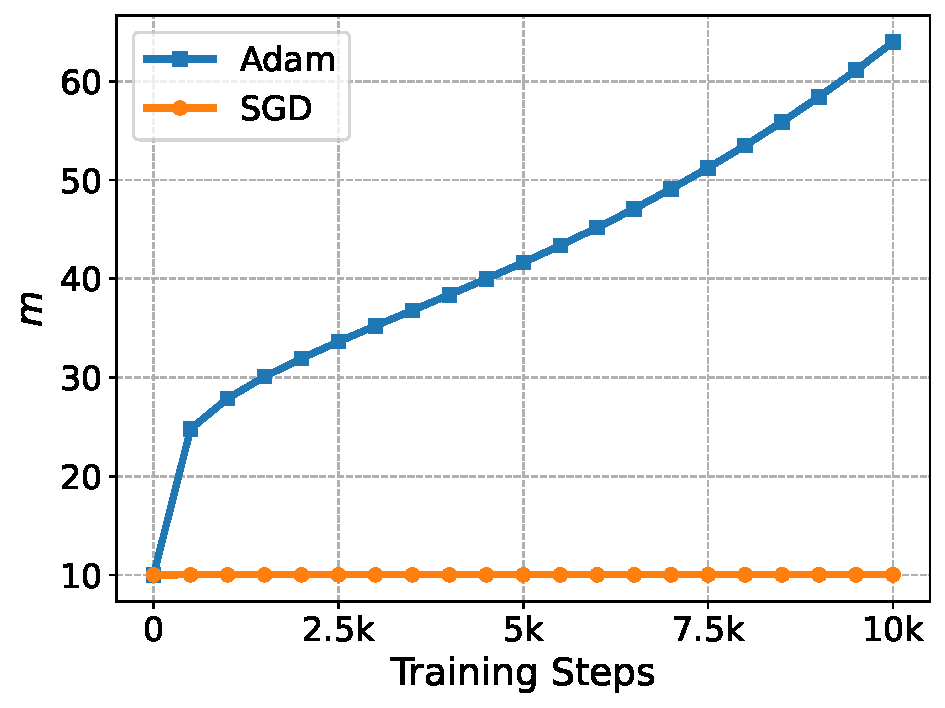
\includegraphics[width=0.5\linewidth]{Figures/BBM_appendix/m_dynamics.pdf}
    \caption{With the gradient formula in Proposition~\ref{appthm:massive}, Adam causes linear growth of $m$. 
    % \tianyu{put SGD plot here}
    }
    \label{appfigure:m_dynamics}
\end{figure}